\documentclass[tikz,border=6pt]{standalone}
\usepackage[T1]{fontenc}
\usepackage{lmodern}
\usetikzlibrary{arrows.meta,backgrounds}
\begin{document}
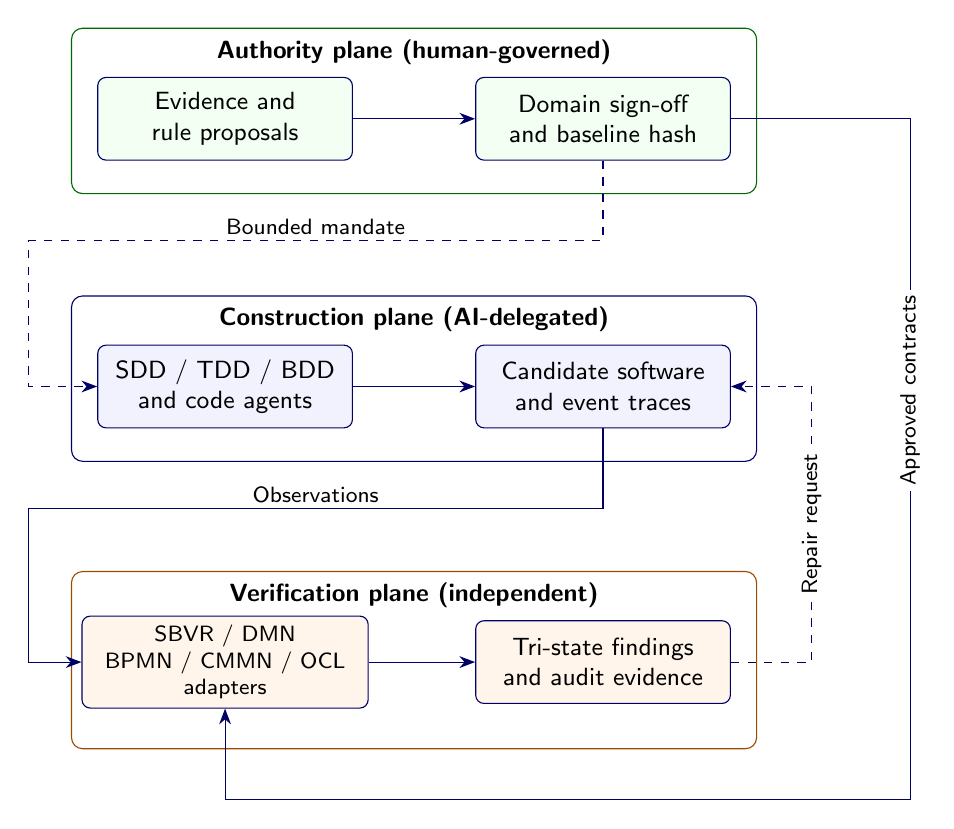
\begin{tikzpicture}[
  font=\sffamily\small,
  box/.style={draw=blue!40!black,rounded corners=3pt,
    align=center,text width=3cm,minimum height=1.05cm,fill=white},
  flow/.style={-{Stealth[length=2mm]},draw=blue!40!black},
  note/.style={font=\sffamily\footnotesize,fill=white,inner sep=2pt,align=center}
]
\node[box,fill=green!5] (evidence) at (0,0) {Evidence and\\rule proposals};
\node[box,fill=green!5] (approval) at (4.8,0) {Domain sign-off\\and baseline hash};
\node[box,fill=blue!5] (builder) at (0,-3.4) {SDD / TDD / BDD\\and code agents};
\node[box,fill=blue!5] (candidate) at (4.8,-3.4) {Candidate software\\and event traces};
\node[box,fill=orange!8,font=\sffamily\footnotesize,text width=3.4cm] (adapters) at (0,-6.9) {SBVR / DMN\\BPMN / CMMN / OCL\\adapters};
\node[box,fill=orange!8] (findings) at (4.8,-6.9) {Tri-state findings\\and audit evidence};

\begin{scope}[on background layer]
\draw[green!40!black,rounded corners] (-1.95,1.15) rectangle (6.75,-.95);
\draw[blue!40!black,rounded corners] (-1.95,-2.25) rectangle (6.75,-4.35);
\draw[orange!60!black,rounded corners] (-1.95,-5.75) rectangle (6.75,-8);
\end{scope}
\node[font=\sffamily\bfseries\small] at (2.4,.85) {Authority plane (human-governed)};
\node[font=\sffamily\bfseries\small] at (2.4,-2.55) {Construction plane (AI-delegated)};
\node[font=\sffamily\bfseries\small] at (2.4,-6.05) {Verification plane (independent)};

\draw[flow] (evidence) -- (approval);
\draw[flow] (builder) -- (candidate);
\draw[flow] (adapters) -- (findings);
\draw[flow,dashed] (approval.south) -- (4.8,-1.55)
  -- node[note,above]{Bounded mandate} (-2.5,-1.55)
  -- (-2.5,-3.4) -- (builder.west);
\draw[flow] (approval.east) -- (8.7,0)
  -- node[note,rotate=90]{Approved contracts} (8.7,-6.9)
  -- (8.7,-8.65) -- (0,-8.65) -- (adapters.south);
\draw[flow] (candidate.south) -- (4.8,-4.95)
  -- node[note,above]{Observations} (-2.5,-4.95)
  -- (-2.5,-6.9) -- (adapters.west);
\draw[flow,dashed] (findings.east) -- (7.45,-6.9)
  -- node[note,rotate=90]{Repair request} (7.45,-3.4) -- (candidate.east);
\end{tikzpicture}
\end{document}
